\section{Application of the Abstract Results}\label{sec:applications}
%
We apply the abstract results of Theorems 1 to 4 in this section. We first consider two toy examples -- Euclidean spaces, section \ref{ssec:app:euclid} and infinite dimensional Hilbert spaces, section \ref{ssec:app:hilbert} --  to better understand the result and compare them to optimal bounds. Then we discuss two more involved settings: The Fréchet mean for non-convex subsets of Euclidean spaces, section \ref{ssec:app:nonconvex}, and for Hadamard spaces, section \ref{ssec:app:hadamard}.
%
%
\subsection{Euclidean Spaces}\label{ssec:app:euclid}
%
	Let $\mc Q \subset \R^b$ be convex with the Euclidean metric $d(p,q) = \normof{p-q}$.
	Choose $\mc Y = \mc Q$, $\mf c =  d^2$, $\mf l = d$, $\xi=1$.
	Let $Y$ be a $\mc Q$-valued random variable with $\Ex{\normof{Y}^2}<\infty$.
	Then the Fréchet mean equals the expectation $m =\Ex{Y} \in \mc Q$. We can easily calculate
	\begin{equation*}
		\Ex*{\normof{Y-q}^2-\normof{Y-m}^2} = \normof{q-m}^2\eqfs
	\end{equation*}
	Thus, the \assu{ass:gr}{Growth} condition is fulfilled with $\gamma=2$.
	The space has the strong quadruple inequality at every point with data distance $\mf a(y,z) = 2 \normof{y-z}$ and strong quadruple distance $\mf b_m(p,q) = \normOf{\frac{q-m}{\normof{q-m}}-\frac{p-m}{\normof{p-m}}}$, see section \ref{sssec:inner_product_space}. Thus, \autoref{thm:abstr_rate_exp} implies
	\begin{align*}
		\Ex*{\normOf{\Ex{Y}-\frac1n\sum_{i=1}^nY_i}^2} 
		&=
		\Ex*{\mf l(m,m_n)^2} 
		\\&\leq 
		C
		n^{-1} 
		\entrn(\mc Q, \mf b_m)^2
		\Ex*{\mf a(Y\pr, Y)^2}
		\\&\leq
		C\pr b \frac1n \Ex*{\normOf{Y-\Ex{Y}}^2}
		\eqcm
	\end{align*}
	where we used $N(r,\Ball{R}{0}{d},d) \leq \br{\frac{3 R}{r}}^b$ for all $R>r>0$ \cite[section 4]{pollard90} to fulfill \assu{ass:sent}{Strong Entropy}. The constants $C, C\pr > 0$ are universal.
	Compare this with the result that one obtains by direct calculations, i.e.,
	\begin{equation*}
		\Ex*{\normOf{\Ex{Y}-\frac1n\sum_{i=1}^nY_i}^2}  = \frac1n\Ex*{\normOf{Y-\Ex{Y}}^2}
		\eqfs
	\end{equation*}
	We pay an extra dimension factor $b$ when using the Fréchet mean approach instead of direct calculations. This comes from the use of the Cauchy--Schwartz inequality, which powers the strong quadruple inequality in Euclidean spaces.
%
%
\subsection{Hilbert Spaces}\label{ssec:app:hilbert}
%
	Let $\mb H$ be an infinite dimensional Hilbert space and $\mc Q \subset \mb H$ convex.
	Let $d(p,q)^2 = \normof{p-q}^2 = \ip{p-q}{p-q}$.
	Choose $\mc Y = \mc Q$, $\mf c =  d^2$, $\mf l = d$, $\xi=1$.
	Let $Y$ be a $\mc Q$-valued random variable with $\Ex{\normof{Y}^2}<\infty$.
	As in the Euclidean case, the Fréchet mean $m$ equals the expectation $\Ex{Y}$, the \assu{ass:gr}{Growth} condition holds with $\gamma=2$, and the strong quadruple inequality is fulfilled with $\mf a(y,z) = 2 \normof{y-z}$ and pseudometric $\mf b_m(p,q) = \normOf{\frac{q-m}{\normof{q-m}}-\frac{p-m}{\normof{p-m}}}$.
	
	Unfortunately, \assu{ass:sent}{Strong Entropy} is not fulfilled on $\mb H$ if $\dim(\mb H) = \infty$. 
	By introducing a weight sequence, we can make $\mf b_m$ smaller by making $\mf a$ larger: 
	Assume that the Hilbert space $\mb H$ is separable and thus admits a countable basis. Let $s=(s_k)_{k\in\N} \subset(0,\infty)$.
	In section \ref{sssec:inner_product_space}, we derived that the strong quadruple condition holds with
	$\mf a(y,z) = 2\normof{y-z}_{s^{-1}}$ and $\mf b_m^s (p,q)=  \normOf{\frac{q-m}{\normof{q-m}}-\frac{p-m}{\normof{p-m}}}_{s}$.
	Then $\entrn(\mb H, \mf b_m^s) \leq \gamma_2(\mb H, \mf b_m^s) \leq \gamma_2(\mc E_s, d)$, where 
	\begin{equation*}
		\mc E_s = \cb{h\in\mb H \colon \sum_{k=1}^\infty \frac{h_k^2}{s_k^2}\leq 1}
		\eqfs
	\end{equation*}
	There is a universal constant $c>0$ such that $\gamma_2(\mc E_s, d)^2 \leq c \sum_{k=1}^\infty s_k^2$, see \cite[Proposition 2.5.1]{talagrand14}.
	As a condition on the variance term, we need
	\begin{equation*}
		\Ex*{\normof{Y-\Ex{Y}}_{s^{-1}}^2} = \normof{\sigma}_{s^{-1}}^2 = \sum_{k=1}^\infty \sigma^2_k s_k^{-2}< \infty
		\eqcm
	\end{equation*}
	where $\sigma^2_k := \VOf{Y_k}$ and $\sigma = (\sigma_k)_{k\in\N}$.
	Similar to the Euclidean case, \autoref{thm:abstr_rate_exp} implies
	\begin{equation*}
		\Ex*{\normOf{\Ex{Y}-\frac1n\sum_{i=1}^nY_i}^2} 
		=
		\Ex*{\mf l(m,m_n)^2} 
		\leq
		C \frac1n \normof{s}_{\ell_2}^2 \normof{\sigma}_{s^{-1}}^2
		\eqcm
	\end{equation*}
	where $\normof{s}_{\ell_2}^2 = \sum_{k=1}^\infty s_k^2$.
	
	Direct calculations yield a better result:
	\begin{equation*}
		\Ex*{\normOf{\Ex{Y}-\frac1n\sum_{i=1}^nY_i}^2} 
		=
		\frac1n \normof{\sigma}_{\ell_2}^2
		\eqfs
	\end{equation*}
	As in the Euclidean case, we pay a factor related to the dimension for using the more generally applicable Fréchet mean approach instead of using the inner product for direct calculations.
%
%
\subsection{Non-Convex Subsets}\label{ssec:app:nonconvex}
%
	Assume we are in the setting of section \ref{ssec:app:hilbert} and the mentioned conditions for convergence are fulfilled.
	But now we want to take $\mc Q \subset \mb H$ not necessarily convex and $\mc Y = \mb H$. Assume that \assu{ass:ex}{Existence} of the Fréchet mean $m\in\mc Q$ is fulfilled. The expectation $\mu := \Ex{Y} \in \mb H$ might not be an element of $Q$. Then the Fréchet mean $m$ is the closest projection of $\mu$ to $\mc Q$, in the sense that
	\begin{align*}
		\argmin_{q\in\mc Q} \Ex{\normof{Y-q}^2} 
		= 
		\argmin_{q\in\mc Q} \normof{\mu-q}
		\eqfs
	\end{align*}
	To get the same rate as in section \ref{ssec:app:hilbert}, we mainly need to be concerned with the \assu{ass:gr}{Growth} condition, as the quadruple condition holds in all subsets.
	For $q\in\mb H$, simple calculations show
	\begin{align*}
		\Ex*{\normof{Y-q}^2-\normof{Y-m}^2} 
		=
		\normof{\mu-q}^2-\normof{\mu-m}^2
		\eqfs
	\end{align*}
	We want to find a lower bound of this term in the form of $c_{\ms g} \normof{q-m}^\gamma$ for constants $\gamma, c_{\ms g} > 0$.
	For $a>1$, we have
	\begin{align*}
		&a\normOf{\mu-q}^2-a\normOf{\mu-m}^2 - \normOf{q-m}^2 
		\\&= (a-1)\normOf{q-\br{\mu+\frac{\mu-m}{a-1}}}^2 - \frac{a^2}{a-1} \normOf{m-\mu}^2
		\eqfs
	\end{align*}
	Thus, $\normOf{\mu-q}^2-\normOf{\mu-m}^2 \geq \frac1a\normOf{q-m}^2$ if and only if 
	\begin{equation*}
		\normOf{q-\br{\mu+\frac{\mu-m}{a-1}}} \geq \frac{a}{a-1} \normOf{\mu-m}
		\eqfs
	\end{equation*}
	Equivalently, the \assu{ass:gr}{Growth} condition holds with $\gamma=2$ and $c_{\ms g} \in (0,1)$ if and only if
	\begin{equation*}
		\normOf{q-\br{\mu+\frac{c_{\ms g}}{1-c_{\ms g}} \br{\mu-m}}} \geq \frac{1}{1-c_{\ms g}} \normOf{\mu-m}
	\end{equation*}
	for all $q\in\mc Q$, i.e., if and only if $\mc Q \cap \ball_{r}(p) = \emptyset$, where $r= \frac{1}{1-c_{\ms g}} \normOf{\mu-m}$ and $p=\mu+\frac{1-c_{\ms g}}{c_{\ms g}} \br{\mu-m}$.  Note that $\normof{p-m} = r$.
	%
	\begin{figure}
	\begin{center}
		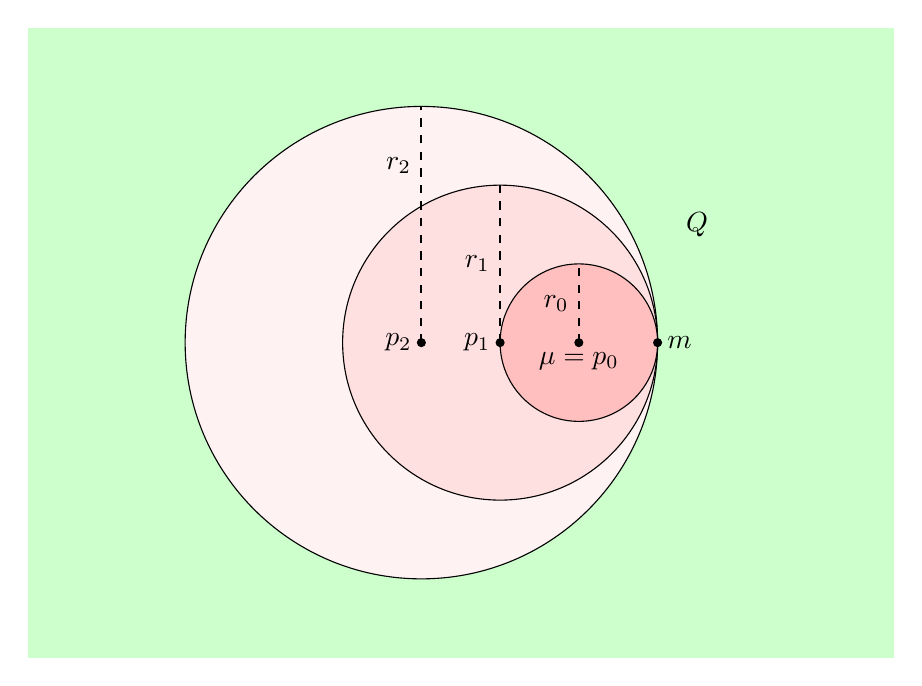
\begin{tikzpicture}
			\fill[green!20!white] (-7,-4) rectangle (4,4);
			\draw[fill=red!5!white] (-2,0) circle (3);
			\draw[fill=red!12!white] (-1,0) circle (2);
			\draw[fill=red!25!white] (0,0) circle (1);
			\filldraw (0,0) circle (0.05) node[below] {$\mu = p_0$};
			\filldraw (1,0) circle (0.05) node[right] {$m$};
			\filldraw (-1,0) circle (0.05) node[left] {$p_1$};
			\filldraw (-2,0) circle (0.05) node[left] {$p_2$};
			\draw[thick,dashed] (0,0) -- node[left]{$r_0$} (0,1);
			\draw[thick,dashed] (-1,0) -- node[left]{$r_1$} (-1,2);
			\draw[thick,dashed] (-2,0) -- node[near end, left]{$r_2$} (-2,3);
			\node at (1.5,1.5) {$\mc Q$};
		\end{tikzpicture}
	\end{center}
	\caption{If $\mc Q \cap \ball_{r_0}(p_0) \neq \emptyset$, the point $m$ cannot be the Fréchet mean of a distribution with expectation $\mu$. To fulfill the 
	%	\assu{ass:gr}{Growth}
	\texttt{Growth}
	condition, we need $\mc Q \cap \ball_{r_1}(p_1) = \emptyset$ for a ball with larger radius $r_1 > r_0$ and adjusted center $p_1$. Increasing the radius further, $r_2>r_1$, only improves the constant $c_{\ms g}$ of the 
	%	\assu{ass:gr}{Growth} 
	\texttt{Growth}
	condition, but not the exponent $\gamma$.
	}\label{fig:nonconvsubset}
	\end{figure}
	%
	This is illustrated in \autoref{fig:nonconvsubset}.
	We have answered the question of how $\mc Q$ may look like, given the location of $\mu$ and $m$. Possibly more interesting is the question of, given $\mc Q$, where may $\mu$ be located so that $m$ can be estimated with the same rate as for convex sets. We will answer this question only informally via a description similar to a \textit{medial axis transform} \cite{choi97}:
	
	For simplicity assume $\mc Q = \R^2 \setminus A$, where $A$ is a nonempty, open, and simply connected set with border $\partial A$ that is parameterized by the continuous function $\gamma\colon[0,1] \to \partial A$. Roll a ball along the border on the inside of $A$. Make the ball as large as possible at any point so that it is fully contained in $A$ and touches the border at point $\gamma(t)$. Denote the center of the ball as $c \colon [0,1]\to A$ and the radius as $r \colon [0,1] \to [0,\infty)$. Take $\epsilon\in(0,1)$ and trace the point $p_\epsilon\colon[0,1]\to A$ on the radius connecting the center of the ball $c(t)$ and the border $\gamma(t)$ such that it divides the radius into two pieces of length $\ol {p_\epsilon(t)}{c(t)} = \epsilon r(t)$ and $\ol {p_\epsilon(t)}{\gamma(t)} =(1-\epsilon) r(t)$. If $\mu$ lies on the outside of the set prescribed by $p\colon[0,1]\to A$, it can be estimated with the same rate as for convex sets.
	This is illustrated in \autoref{fig:nonconvxheart}.
	%
	\begin{figure}
		\begin{center}
			\includegraphics[width=0.8\textwidth]{nonconvex_heart.pdf}
		\end{center}
		\caption{Let $A\subset\R^2$ be the set enclosed by the heart (solid black lines). Let $\mc Y = \R^2$ and $\mc Q = \R^2 \setminus A$. We consider a distribution on $\R^2$ with mean $\mu\in\mc Y$ and Fréchet mean $m\in\mc Q$ with respect to the Euclidean metric and the descriptor space $\mc Q$. The green, blue, and red lines show $p_\epsilon(t)$ for $\epsilon = 0.6, 0.3, 0$.}\label{fig:nonconvxheart}
	\end{figure}
	%
	The set of all centers $\mc C := \cb{c(t) \,|\, t \in [0,1]}$, also called the \textit{medial axis} ot \textit{cut locus}, is critical: The closer $\mu$ is to $\mc C$, the larger the guaranteed error bound for the estimator. In particular, we cannot guarantee consistency of  the estimator if $\mu \in \mc C$. A very similar phenomenon is described in \cite[section 3]{bhattacharya03}. The authors consider a Riemannian manifold $\mc Q$ that is embedded in an Euclidean space $\mc Y$. The \textit{extrinsic mean} of a distribution on $\mc Q$ is the projection of the mean $\mu$ in $\mc Y$ to $\mc Q$. The points $\mc C$ are called \textit{focal points}. It is shown \cite[Theorem 3.3]{bhattacharya03} that in many cases the \textit{intrinsic mean}, i.e, the Fréchet mean in $\mc Q$ with respect to the Riemannian metric on $\mc Q$, is equal to the extrinsic mean, i.e, the Fréchet mean in $\mc Q$ with respect to the Euclidean metric on $\mc Y$.
	
	The conditions described above are connected to the term reach of a set \cite{federer59}. The reach of $\mc Q \subset \R^b$ is the largest $\epsilon>0$ (possibly $\infty$) such that $\inf_{q\in\mc Q} d(x, q) < \epsilon$ implies that $x \in \R^b$ has a unique projection to $\mc Q$, i.e., a unique point $x_\mc Q$ with $d(x, x_{\mc Q}) = \inf_{q\in\mc Q} d(x, q)$. If the distance of the mean $\mu$ to $\mc Q$ is less than the reach of $\mc Q$, then the \assu{ass:gr}{Growth} condition holds with $\gamma = 2$. Thus, the rate of convergence is upper bounded by $c n^{-\frac12}$ for some $c>0$. Note that convex sets have infinite reach and exhibit this upper bound for any distribution with finite second moment.

	By considering the growth condition $\normOf{\mu-q}^2-\normOf{\mu-m}^2 \geq c_{\ms g}\normOf{q-m}^\gamma$, one can also find examples of subspaces where the growth exponent for specific distributions is different from 2.
%
%
%
%
\subsection{Hadamard Spaces}\label{ssec:app:hadamard}
%
%
Let $(\mc Q, d)$ be a Hadamard space. A definition of Hadamard spaces is given in section \ref{ssse:quad:npc}. Use the notation $\ol yq = d(y,q)$. For our purposes the most notable property of Hadamard spaces is that they fulfill the nice quadruple property, i.e., $\ol yq^2 - \ol yp^2 - \ol zq^2 + \ol zp^2 \leq 2 \,\ol yz\, \ol qp$. In the following subsections, we will see how this translates to convergence rates for the Fréchet mean estimator and use the power inequality to obtain results for a generalized Fréchet mean with cost function $d^{2a}$ for $a\in[\frac12, 1]$.

For an introduction to Hadamard spaces see \cite{bacak14}. A survey of recent developments can be found in \cite{bacak18}. 
In \cite{berg08} the authors characterize Hadamard spaces by the nice quadruple inequality and discuss a quasilinearzation of these spaces by observing that the left hand side of the nice quadruple inequality behaves like an inner product to some extend. \cite{sturm03} shows how some important theorems of probability theory in Euclidean spaces, like the law of large numbers and Jensen's inequality, translate to non-Euclidean Hadamard spaces. In \cite{sturm02} martingale theory on Hadamard spaces is discussed.

Turning to more applied topics, \cite{bacak14b} shows algorithms for calculating the Fréchet mean in Hadamard spaces with cost function $d^{2a}$ for $a=\frac12$ and $a=1$.
An important application of Hadamard spaces in Bioinformatics are phylogenetic trees \cite{billera01}. See also \cite[section 6.3]{bacak18} for a quick overview. Another application of Hadamard spaces is taking means in the manifold of positive definite matrices, e.g., in diffusion tensor imaging. But note that, as the underlying space is a differentiable manifold, one an use gradient-based approaches, see \cite{pennec06}.

Further examples of Hadamard spaces include Hilbert spaces, the Poincaré disc, complete metric trees, complete simply-connected Riemannian manifolds of nonpositive sectional curvature. See also \cite[section 3]{sturm03}.
%
%
%
\subsubsection{Fréchet Mean}\label{sssec:app:hadamard:fm}
%
Let $(\mc Q, d)$ be a Hadamard space. We use $\mc Q$ as data space as well as descriptor space, i.e., $\mc Q = \mc Y$. The cost function is $\mf c=d^2$, the loss $\mf l = d$. As described in section  \ref{ssse:quad:npc} the weak quadruple inequality holds with $\mf a = 2d$ and $\mf b = d$, i.e., $(\mc Q,d)$ fulfills the nice quadruple inequality.
Let $Y$ be a random variable with values in $\mc Q$. Let $Y_1, \dots, Y_n$ be iid copies of $Y$.

If $\Ex{d(Y,q)^2} < \infty$ for one $q\in\mc Q$, then it is also finite for every $q\in\mc Q$ and the Fréchet mean $m\in\argmin_{q\in\mc Q} \Ex{d(Y,q)^2}$ exists and is unique, see \cite[Proposition 4.3]{sturm03}. The same holds true for the estimator $m_n\in\argmin_{q\in\mc Q} \sum_{i=1}^n{d(Y_i,q)^2}$. Thus, \assu{ass:ex}{Existence} is fulfilled.

Here, we chose a second moment condition, because we will need it for estimation anyway. But note that choosing the cost function as $\mf c(y,q) = d(y,q)^2 - d(y,o)^2$ for a fixed, arbitrary point $o\in\mc Q$ allows us to require only a finite first moment for \assu{ass:ex}{Existence} and the resulting Fréchet mean coincides with the $d^2$-Fréchet mean if the second moment is finite. This is described in more detail and utilized in \cite{sturm03}.

Furthermore, the \assu{ass:gr}{Growth}-condition holds in Hadamard spaces with $\gamma=2$ and $c_{\ms g} = 1$, see \cite[Proposition 4.4]{sturm03}.
%
Thus, we obtain following corollary of \autoref{thm:abstr_rate_prob}.
%
\begin{corollary}[Convergence rate in probability]
	Assume \assu{ass:mom}{Moment} with $\zeta = 2$ and $\mf a = 2d$ and \assu{ass:ent}{Entropy}  with $\mf b = d$ and $\alpha=\beta$.
	Define
	\begin{equation*}
		\eta_{\beta,n} := 
		\begin{cases} 
			n^{-\frac12} & \text{ for }\beta < 1\eqcm\\
			n^{-\frac12} \log(n+1) & \text{ for } \beta = 1\eqcm\\
			n^{-\frac1{2\beta}} & \text{ for } \beta > 1\eqfs
		\end{cases} 
	\end{equation*}
	Then, for all $s > 0$, we have
	\begin{equation*}
		\PrOf{\eta_{\beta,n}^{-1} d(m,m_n) \geq s} \leq c \,\Ex{d(Y,Y\pr)^2} \,s^{-2}
		\eqcm
	\end{equation*}
	with a constant $c > 0$ depending only on $\beta$ and $c_{\ms e}$.
	In particular,
	\begin{equation*}
		d(m, m_n) = \bigOp\brOf{\eta_{\beta,n}}
		\eqfs
	\end{equation*}
\end{corollary}
%
As described in section \ref{ssse:quad:npc}, it may be difficult to find a version of the strong quadruple inequality such that the same rate can be derived for convergence in expectation. Thus, instead of trying to apply \autoref{thm:abstr_rate_exp}, we utilize (i) \autoref{cor:probtoexpec} and (ii) \autoref{thm:abstr_weak_strong}, respectively.
%
\begin{corollary}
\theoremContentInNewLine
	\begin{enumerate}[label=\environmentEnumerateLabel]
	\item 
		Let $\epsilon > 0$.
		Assume $\Ex*{d(Y,Y\pr)^{2+\epsilon}} < \infty$.
		Assume \assu{ass:ent}{Entropy}  with $\mf b = d$ and $\alpha=\beta < 1$.
		Then we have
		\begin{equation*}
			\Ex*{d(m, m_n)^2} \leq c\, \Ex*{d(Y,Y\pr)^{2+\epsilon}}^{\frac{2}{2+\epsilon}} \,\frac1{\epsilon n }
		\end{equation*}
		for a constant $c>0$ depending only on $\beta$.
	\item 
		Assume $\Ex*{d(Y,Y\pr)^2} < \infty$.
		Let $o\in\mc Q$. Assume \assu{ass:se}{Small Entropy} with $\mf b = d$.
		Let $\tilde m_n \in \argmin_{q\in\ball_n(o)} \sum_{i=1}^n d(Y_i, q)^2$.
		Then we have
		\begin{equation*}
			\Ex*{d(m, \tilde m_n)^2} = \bigO\brOf{\frac1n \log(n)^{2\beta}}
			\eqfs
		\end{equation*}
	\end{enumerate}
\end{corollary}
%
%
\subsubsection{Power Fréchet Mean}\label{sssec:app:hadamard:pfm}
%
We go beyond Hadamard spaces by utilizing the power inequality, \autoref{thm:power_inequ}. 
Let $(\mc Q, d)$ is a Hadamard space and $a \in[\frac12,1)$. Then $(\mc Q, d^a)$ is not Hadamard, but fulfills a weak quadruple inequality: Fix an arbitrary point $o\in\mc Q$. We use the cost function $\mf c(y,q) = d^{2a}(y,q)-d^{2a}(y,o)$ and the loss $\mf l = d$. Then the weak quadruple inequality holds with $\mf a (y,z) = 8a2^{-2a} d(y,z)^{2a-1}$ and $\mf b = d$.

We need to choose the cost function $d^{2a}(y,q)-d^{2a}(y,o)$ instead of $d^{2a}(y,q)$ to obtain a result with minimal moment requirement. To fulfill \assu{ass:mom}{Moment} we need $\Ex{d(Y,Y\pr)^{2(2a-1)}} < \infty$ and for \assu{ass:ex}{Existence}, we need $\Ex{\abs{\mf c(Y,q)}} < \infty$. We fulfill both by assuming that
$\Ex{d(Y,o)^{2(2a-1)}} < \infty$. Then the both conditions are satisfied: On one hand
$\Ex{d(Y,Y\pr)^{2(2a-1)}} \leq 2 \Ex{d(Y,o)^{2(2a-1)}}$. On the other hand, using 
the tight power bound of \autoref{lmm:tightpowerbound} (appendix \autoref{app:power_inequality}),
\begin{align*}
	\ol yq^{2a}-\ol yo^{2a}
	\leq 
	2 a \,\ol qo \br{\frac{\ol yq + \ol yo}{2}}^{2a-1}
\end{align*} 
and thus 
\begin{equation*}
	|\mf c(Y,q)|  \leq 2a \,\ol qo \br{\frac{\ol qo}{2} +  \ol Yo}^{2a-1}\eqcm
\end{equation*}
which implies 
$\Ex{\abs{\mf c(Y, q)}} < \infty$. But $\Ex{d(Y,q)^{2a}}$ might be infinite as $2a > 2(2a-1)$.

\autoref{thm:abstr_rate_prob} with $\zeta=2$ implies following corollary.
%
\begin{corollary}[Rates in probability for power mean]\label{coro:probrates_power}
	Assume:
	\begin{enumerate}[label=\environmentEnumerateLabel]
	\item
		\assu{ass:ex}{Existence}:	Let $a\in[\frac12,1]$. Let $o\in\mc Q$ be an arbitrary fixed point. Assume there are $m_n\in\argmin_{q\in\mc Q} \frac1n\sum_{i=1}^n \br{\ol{Y_i}{q}^{2a}-\ol {Y_i}o^{2a}}$ measurable and $m\in\argmin_{q\in\mc Q} \Ex{\ol Yq^{2a}-\ol Yo^{2a}}$.
	\item 
		\assu{ass:gr}{Growth}: There are constants $c_{\ms g} > 0, \gamma\in(1,\infty)$ such that 
				$\Ex{\ol Yq^{2a}}-\Ex{\ol Ym^{2a}}  \geq c_{\ms g} d(m,q)^\gamma$ for all $q\in\mc Q$.
	\item \assu{ass:mom}{Moment}:   $\Ex{\ol{Y}{q}^{2(2a-1)}} < \infty$ for one (and thus for all) $q\in\mc Q$.
	\item \assu{ass:ent}{Entropy}: 
		There is $\beta > 0$ such that
		\begin{equation*}
			\sqrt{\log N(\ball_\delta(m, d), d, r)} \leq c_{\ms e} \br{\frac{\delta}{r}}^\beta
		\end{equation*}
		for all $\delta, r > 0$.
	\end{enumerate}
	Then, for all $s > 0$, we have
	\begin{equation*}
		\PrOf{\eta_{\beta,n}^{-\frac1{\gamma-1}}\, \ol{m}{m_n} \geq s} \leq c \,\Ex{\ol{Y}{o}^{2(2a-1)}} \, s^{-2(\gamma-1)}
		\eqcm
	\end{equation*}
	where $c > 0$ depends only on $\beta, \gamma, c_{\ms e}$.
	In particular,
	\begin{equation*}
		d(m, m_n) = \bigOp\brOf{\eta_{\beta,n}^{-\frac1{\gamma-1}}}
		\eqfs
	\end{equation*}
\end{corollary}
%
Note that the moment condition becomes weaker as $a$ gets smaller and vanishes for $a=\frac12$, where, in the Euclidean case, the Fréchet mean is the median. 

\assu{ass:ex}{Existence} of $m_n$ and $m$ is a purely technical condition, as one will usually only be able to minimize the objective functions up to an $\epsilon>0$ and the set of $\epsilon$-minimizers is always nonempty.

The \assu{ass:gr}{Growth} condition is more interesting. It seems possible to choose $\gamma=2$ for all $a\in[\frac12,1]$ in many circumstances, at least under some conditions on the distribution of $Y$. But precises statements of this sort are unknown to the author. If $\gamma$ really can be chosen independently of $a$, then the rate is the same for all $a\in[\frac12,1]$. In the Euclidean case, this is manifested in the fact that we can estimate median ($a = \frac12$) and mean ($a = 1$) and all statistics ``in between" ($a \in (\frac12,1)$) with the same rate (under some conditions), but with less restrictive moment assumptions for smaller powers $a$.

Similarly to the corollary above, we can apply \autoref{cor:probtoexpec} or \autoref{thm:abstr_weak_strong} to obtain rates in expectation.
%
%
%
%
%